\documentclass[12pt]{article}

%AMS-TeX packages
\usepackage{amssymb,amsmath,amsthm} 
\usepackage{geometry, graphicx}
\usepackage{tabulary}
\usepackage{upgreek}
\usepackage{siunitx}
\usepackage{caption}
\usepackage{subcaption}
\usepackage{csvsimple}
\usepackage{enumitem}


\usepackage{pgfplotstable}
\pgfplotsset{compat=1.9}% supress warning

% setup the margins
\geometry{margin=1.0in, headheight=15pt}

\graphicspath{ {../lab03/images} }    


\begin{document}

\title{PHSX 444: Lab 03; Optical Trapping of Dielectric Particles in Liquid}
\author{William Jardee}
\maketitle

%% Introduction section. Here I introduce the physics of the experiment and give some slight motivation for the experiment. I personally think that putting the physics of the apparatus here is better. 
\section{Introduction}
The purpose of this experiment was to have an introductory to particle trapping, specifically optical particle trapping. A laser, passed through a single mode fiber and culminated, is focused to a point at the end of a microscope objective. Under the objective a solution of water and clear polyethylene microspheres, which will be the target of this optical trap. These microspheres are around 1 $\mu$m - 1.7 mm in diameter, have a density very comparable to water (0.97 g/cm$^3$) and, most importantly, and dielectric \cite{microspheres}. 

When the light hits the microsphere, the dielectric particle is attracted towards the increased electric field, from the EM wave. As it sits in this position, the rays traveling through it stabilize the height; allowing the scattering and reflected light to both push it down when it is above the balanced point, or having the scattering force pushing it down and the reflecting push it up when it is below the balancing point. The way the trap works out, in the latter case the particle is pushed back to the balancing force for small oscillations. With the planar attraction of the E-field, and the height stabilization from the reflection and scattering, particles can effectively be trapped. If this trap is thought of as a curved,  potential well, then then the particle's thermal motion looks like an over-damped oscillator in that well.

The objective of this lab will be to use this method to trap these microspheres to measure their Brownian motion and mass. The Brownian motion can then be used to estimate the strength of the trap and compared against the ``escape velocity" of the trap to analyze the effectiveness of such a simple optical trap. Above these two purposes, the objective of the lab is to become comfortable with the equipment being used, fiddling with optical devices, and using provided code to properly analyze collected data.

\begin{figure}
\centering
    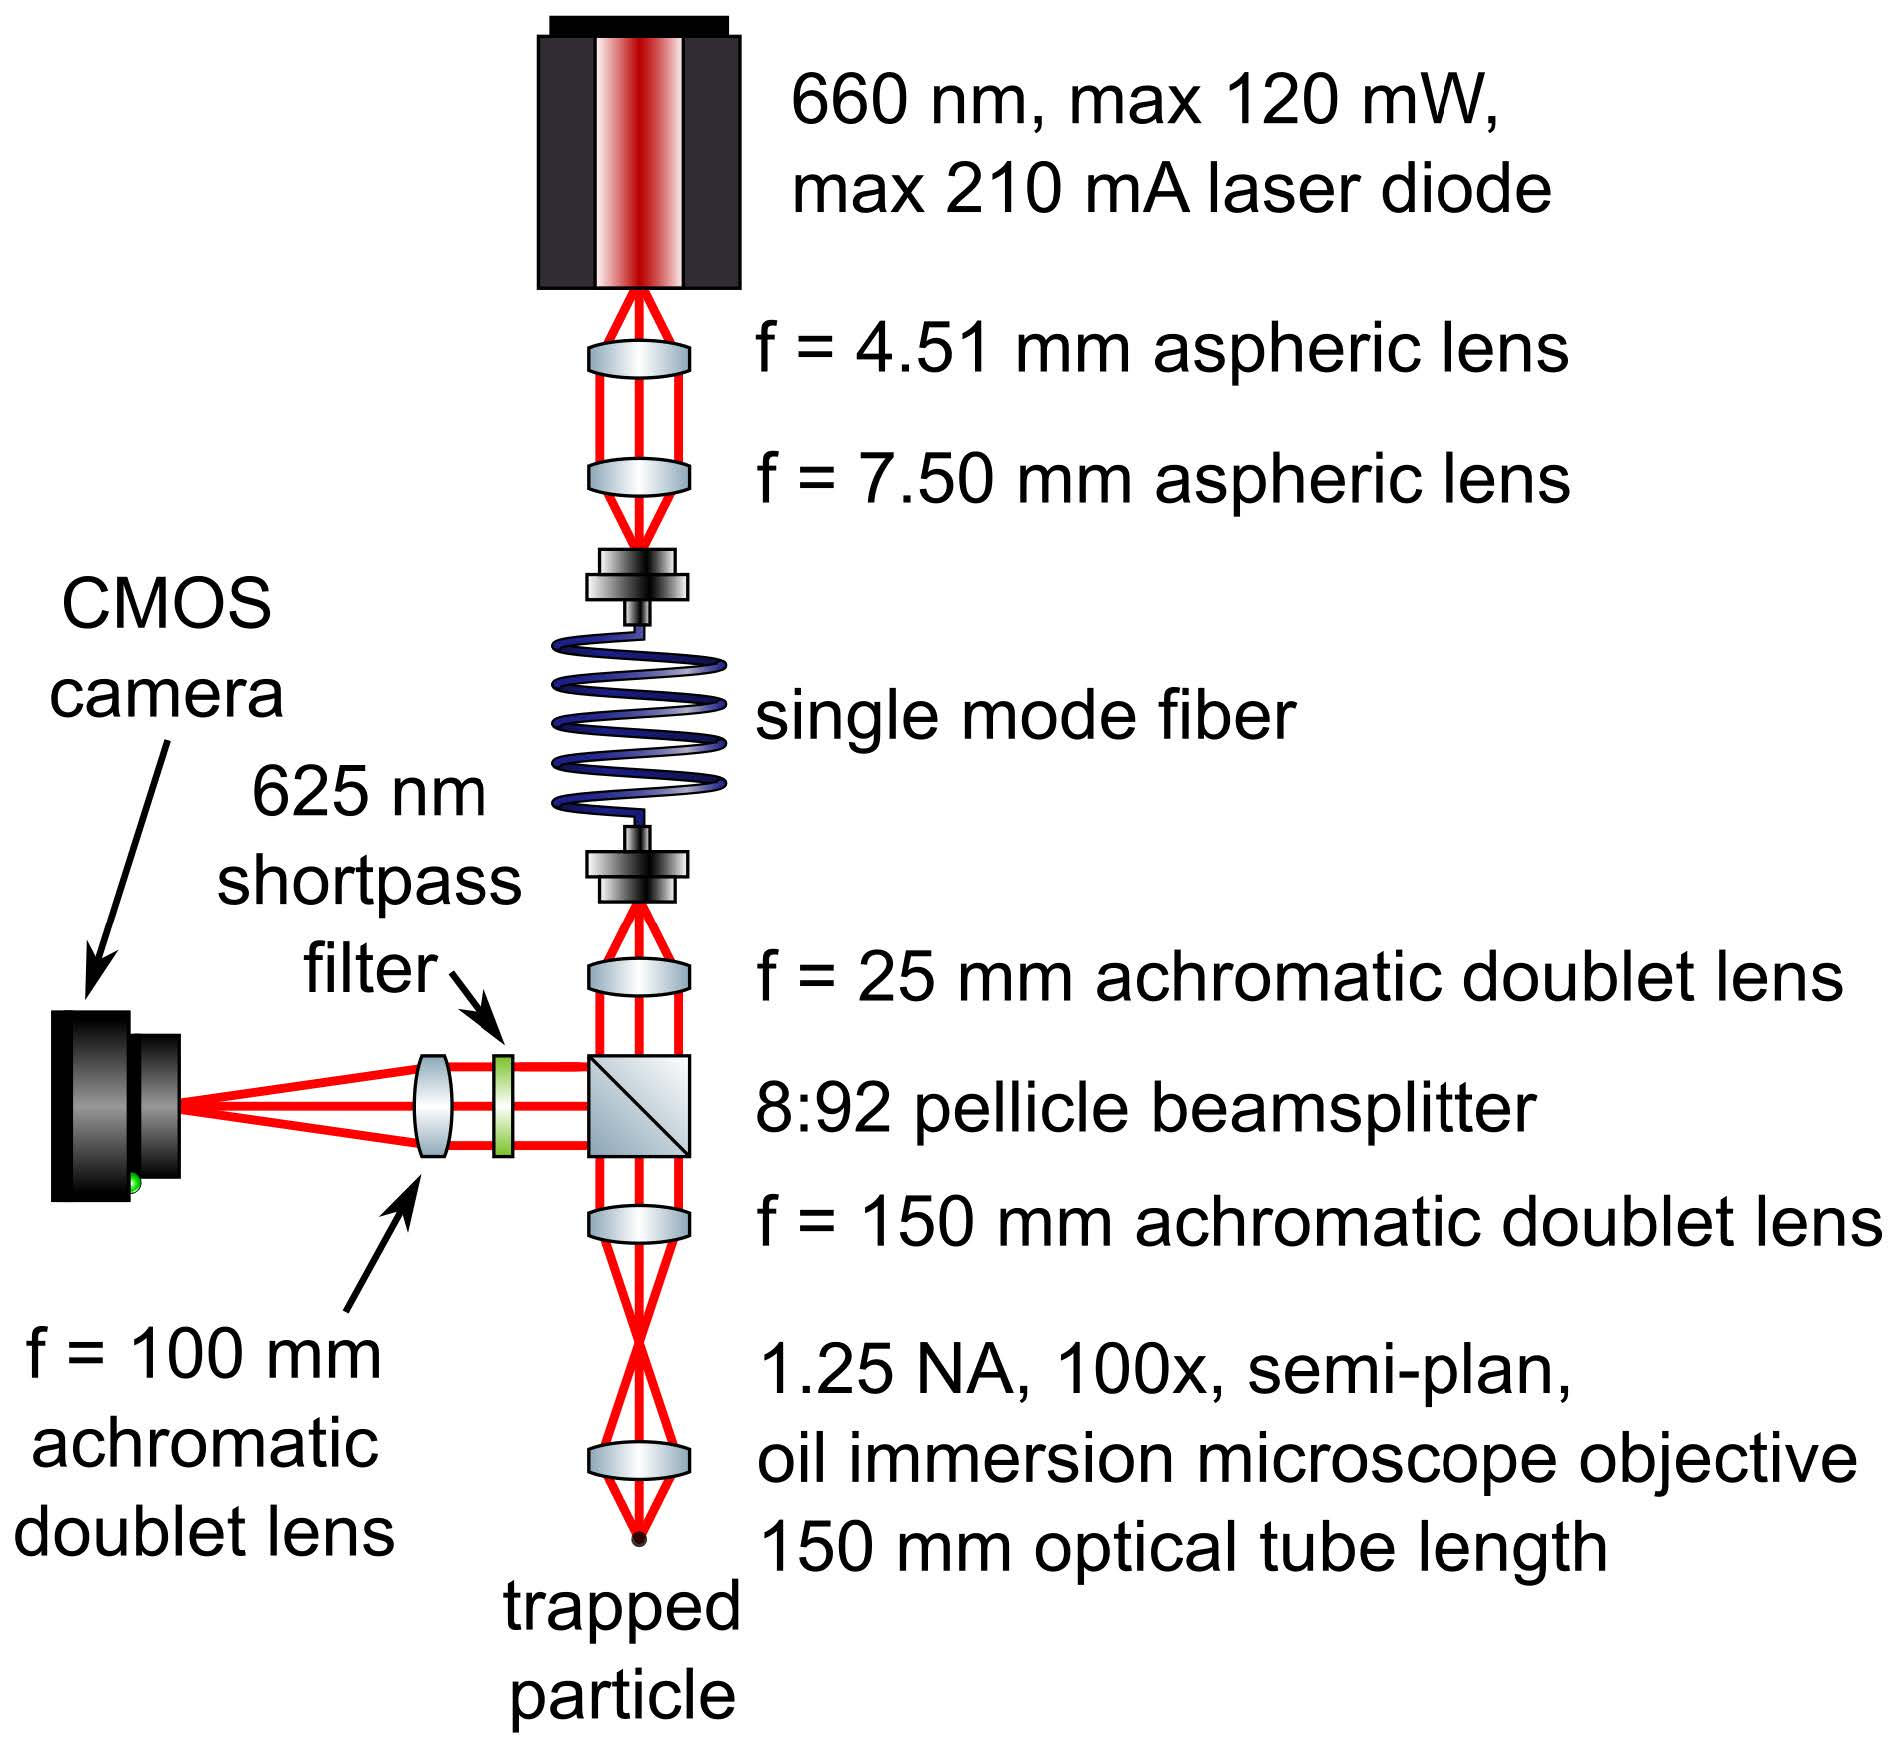
\includegraphics[width=0.5\textwidth]{optical_trap.jpg}
	\caption{\cite{handout}}
    \label{fig:opt_trap}
\end{figure} % optical trap

%% Experimental Methods section. Here I go into depth about the methods used to collect the data. I also talk about where the apparatus came from. I bring up the way that we will be calibrating the data and collecting enough data to do any trend correction later 
\section{Experimental Methods}
This lab was split into three sessions; the first served to dial in the laser and collect calibration data, the second and third served to collect data. 

The first day the laser was dialed in, achieving a power output of about $3.1 \pm 0.2$ mW from a laser diode that was current limited to $67.75$ mA. Focusing this laser into the optical setup seen in Figure~\ref{fig:opt_trap}, the calibration slide was brought into focus to calibrate the camera being used. The calibration gave a pixel size of $128.16126 \text{nm} \times 120 \text{nm}$. This was found by taking a Fourier Transform of the calibration slide and dividing the division by the number of pixel in a period in the primary frequency peak. The orientation used in the calibration picture would be used throughout and this same calibration data will be used both days. 

The second and third sessions served as a continuing improvement on preparing slides with a plethera of microspheres on them and taking many images with them. Some sets of data were as simple as taking video of a particle trapped and showing a random walk. Other sets, of a much longer record period, consisted of ``playing" with the particles to experience the escape velocity, and other interactions such as adding more water to the slide and the consequential current or transfering the current trapped particle to another through a forced collision.

Finally, in post the images taken were able to be cropped down only to the area of interest and processed through a given code that measured the change in position of the particle between frames. Through use of repeated correction, this code was able to get subpixel accuracy of a targeted position of the particle between frames \cite{code paper}. 



%% Results and Analysis section. Here I go into what we actually got out of the tests and the resulting calculations from them. 
\section{Results and Analysis}
\begin{figure}
\centering
    \includegraphics[width=0.5\textwidth]{delta_x.eps}
	\caption{\cite{handout}}
    \label{fig:opt_trap}
\end{figure} % optical trap
\begin{figure}
\centering
    \includegraphics[width=0.5\textwidth]{delta_y.eps}
	\caption{\cite{handout}}
    \label{fig:opt_trap}
\end{figure} % optical trap
\begin{figure}
\centering
    \includegraphics[width=0.5\textwidth]{v_x.eps}
	\caption{\cite{handout}}
    \label{fig:opt_trap}
\end{figure} % optical trap
\begin{figure}
\centering
    \includegraphics[width=0.5\textwidth]{v_y.eps}
	\caption{\cite{handout}}
    \label{fig:opt_trap}
\end{figure} % optical trap


\section{Discussion and Conclusions}

% \bibliographystyle{unsrt}
% \bibliography{references}

% \begin{thebibliography}{1}


% \bibitem{microspheres} https://www.cospheric.com/CPMS_polymer_clear_microspheres_density096.htm

% \bibitem{code paper} % insert paper here.
% \bibitem{handout} % insert paper here.


% \end{thebibliography}
\newpage
\section*{Appendix A}



\end{document}
